\subsection{Descriptive results}

\subsubsection{Trends in interethnic marriage}

\begin{table}[htbp]
    \begin{center}
        \caption{Trends in interethnic marriage at the national level, 1982-2010}
        \label{tab:trends}
        \begin{tabular}{lcccc}
            \hline\hline
                                             & 1982    & 1990    & 2000    & 2010    \\
            \hline
            Intra-ethnic marriage            & 98.11\% & 97.20\% & 96.59\% & 96.30\% \\
            Intermarriage with the Han       & 1.86\%  & 2.75\%  & 3.34\%  & 3.61\%  \\
            Intermarriage between minorities & 0.02\%  & 0.06\%  & 0.07\%  & 0.09\%  \\
            \hline
        \end{tabular}
    \end{center}
\end{table}

We begin by presenting one of the first nationwide accounts of interethnic marriage patterns in China from 1982 to 2010.
Table~\ref{tab:trends} shows that marriages within the same ethnic group dominated throughout the period,
though their share declined from 98.11\% in 1982 to 96.30\% in 2010.
Among interethnic marriages, unions between minorities and Han Chinese were most common,
nearly doubling from 1.86\% to 3.61\% between 1982 and 2010.
Intermarriage between different minority groups, while increasing, remained rare, comprising just 0.09\% of all marriages in 2010.

These nationwide figures are largely a result of differences in ethnic group size.
In our pooled samples, 92.75\% of the married population were Han Chinese,
followed by Southern minorities (3.97\%), Manchu (0.86\%), Hui (0.8\%), Uyghur (0.58\%),
Mongolian (0.48\%), Tibetan (0.30\%), Korean (0.16\%), and Kazakh (0.09\%).
Given these structural constraints, while interethnic marriage rates appear low at the national level,
they may be substantial for individual minority groups.
We therefore turn to examining variations in intermarriage patterns across ethnic groups.

\subsubsection{Variation by gender and ethnic group}

\begin{table}
    \renewcommand{\arraystretch}{1.0}
    \begin{center}
        \caption{Trends in interethnic marriage by gender and ethnic group, 1982-2010}
        \label{tab:trends_ethngrp}
        \begin{tabular}{l rrrr}
            \hline\hline
                         & 1982    & 1990    & 2000    & 2010    \\
            \hline
            Manchu       & 70.10\% & 48.51\% & 48.04\% & 46.34\% \\
            \quad Female & 65.73\% & 44.76\% & 48.39\% & 46.27\% \\
            \quad Male   & 73.48\% & 47.84\% & 48.64\% & 49.71\% \\
            Mongolian    & 26.57\% & 39.69\% & 44.81\% & 45.83\% \\
            \quad Female & 24.11\% & 41.48\% & 48.94\% & 48.03\% \\
            \quad Male   & 28.87\% & 37.79\% & 39.95\% & 43.43\% \\
            Southern     & 13.26\% & 15.77\% & 18.46\% & 19.82\% \\
            \quad Female & 14.58\% & 17.53\% & 21.94\% & 22.28\% \\
            \quad Male   & 11.89\% & 13.93\% & 14.65\% & 17.19\% \\
            Hui          & 10.50\% & 14.78\% & 13.12\% & 12.12\% \\
            \quad Female & 10.12\% & 13.97\% & 13.17\% & 12.52\% \\
            \quad Male   & 10.87\% & 15.58\% & 13.07\% & 11.71\% \\
            Tibetan      & 6.43\%  & 6.64\%  & 10.96\% & 6.35\%  \\
            \quad Female & 7.26\%  & 7.25\%  & 13.17\% & 8.65\%  \\
            \quad Male   & 5.58\%  & 6.03\%  & 8.64\%  & 3.94\%  \\
            Korean       & 2.55\%  & 6.54\%  & 17.92\% & 27.71\% \\
            \quad Female & 3.89\%  & 8.18\%  & 18.52\% & 30.23\% \\
            \quad Male   & 1.16\%  & 4.84\%  & 17.31\% & 25.00\% \\
            Kazakh       & 3.53\%  & 5.81\%  & 3.97\%  & 3.06\%  \\
            \quad Female & 1.93\%  & 5.43\%  & 3.20\%  & 3.48\%  \\
            \quad Male   & 5.08\%  & 6.19\%  & 4.76\%  & 2.63\%  \\
            Han          & 0.99\%  & 1.48\%  & 1.82\%  & 2.00\%  \\
            \quad Female & 1.01\%  & 1.41\%  & 1.54\%  & 1.80\%  \\
            \quad Male   & 0.97\%  & 1.54\%  & 2.10\%  & 2.20\%  \\
            Uyghur       & 0.74\%  & 0.60\%  & 1.02\%  & 0.48\%  \\
            \quad Female & 1.15\%  & 0.80\%  & 1.14\%  & 0.32\%  \\
            \quad Male   & 0.32\%  & 0.40\%  & 0.90\%  & 0.64\%  \\
            \hline
        \end{tabular}
    \end{center}
\end{table}

Table~\ref{tab:trends_ethngrp} presents the changing proportion of interethnic marriages by gender and ethnic group from 1982 to 2010.
By 2010, interethnic marriage was most prevalent among historically more assimilated groups:
the Manchu (46.34\%), Mongolian (45.83\%), and Korean (27.71\%) populations,
followed by Southern minorities (19.82\%), Hui (12.12\%), and Tibetan (6.35\%).
The lowest rates were observed among groups with salient ethnoreligious identities—the Kazakh (3.06\%) and Uyghur (0.48\%)—and the Han majority (2.00\%).
Over the study period, several distinct trends emerged.
The Korean population showed the most dramatic increase in interethnic marriage, from 2.55\% in 1982 to 27.71\% in 2010.
The Han majority's intermarriage rate doubled from 0.99\% to 2.00\%.
Significant increases were also observed among the Mongolian (72.49\% increase) and Southern minorities (49.47\% increase).
In contrast, the Manchu experienced a 33.89\% decrease, with the sharpest decline occurring between 1982 and 1990.

Some groups showed nonlinear trends.
The Hui and Kazakh populations saw initial increases between 1982 and 1990, followed by steady declines.
Intermarriage among Tibetans peaked at 10.96\% in 2000 before returning to 6.35\% in 2010, similar to their 1982-1990 levels.
The Uyghur population maintained consistently low intermarriage rates below 1\%, with a brief exception in 2000.

Gender differences in intermarriage rates varied across ethnic groups.
In some minority populations—such as the Mongolian, Korean, Tibetan, and Southern minorities—women had higher intermarriage rates than men.
For example, in 2010, 8.64\% of Tibetan women married outside their ethnicity, more than double the rate of 3.94\% among Tibetan men.
Similarly, 30.23\% of Korean women intermarried, compared to 25.00\% of Korean men.
Other groups displayed different patterns.
The Hui showed comparable rates between genders, while the Manchu and Han populations had slightly higher rates among men.
The Kazakh and Uyghur groups exhibited notable changes over time.
Among the Kazakh, men initially had higher intermarriage rates (5.08\% versus 1.93\% for women in 1982), but by 2010 these rates had been surpassed by women. The Uyghur population experienced a similar reversal, but in the opposite direction.

\subsubsection{Trends in educational attianment}

\begin{figure}[htbp]
    \centering
    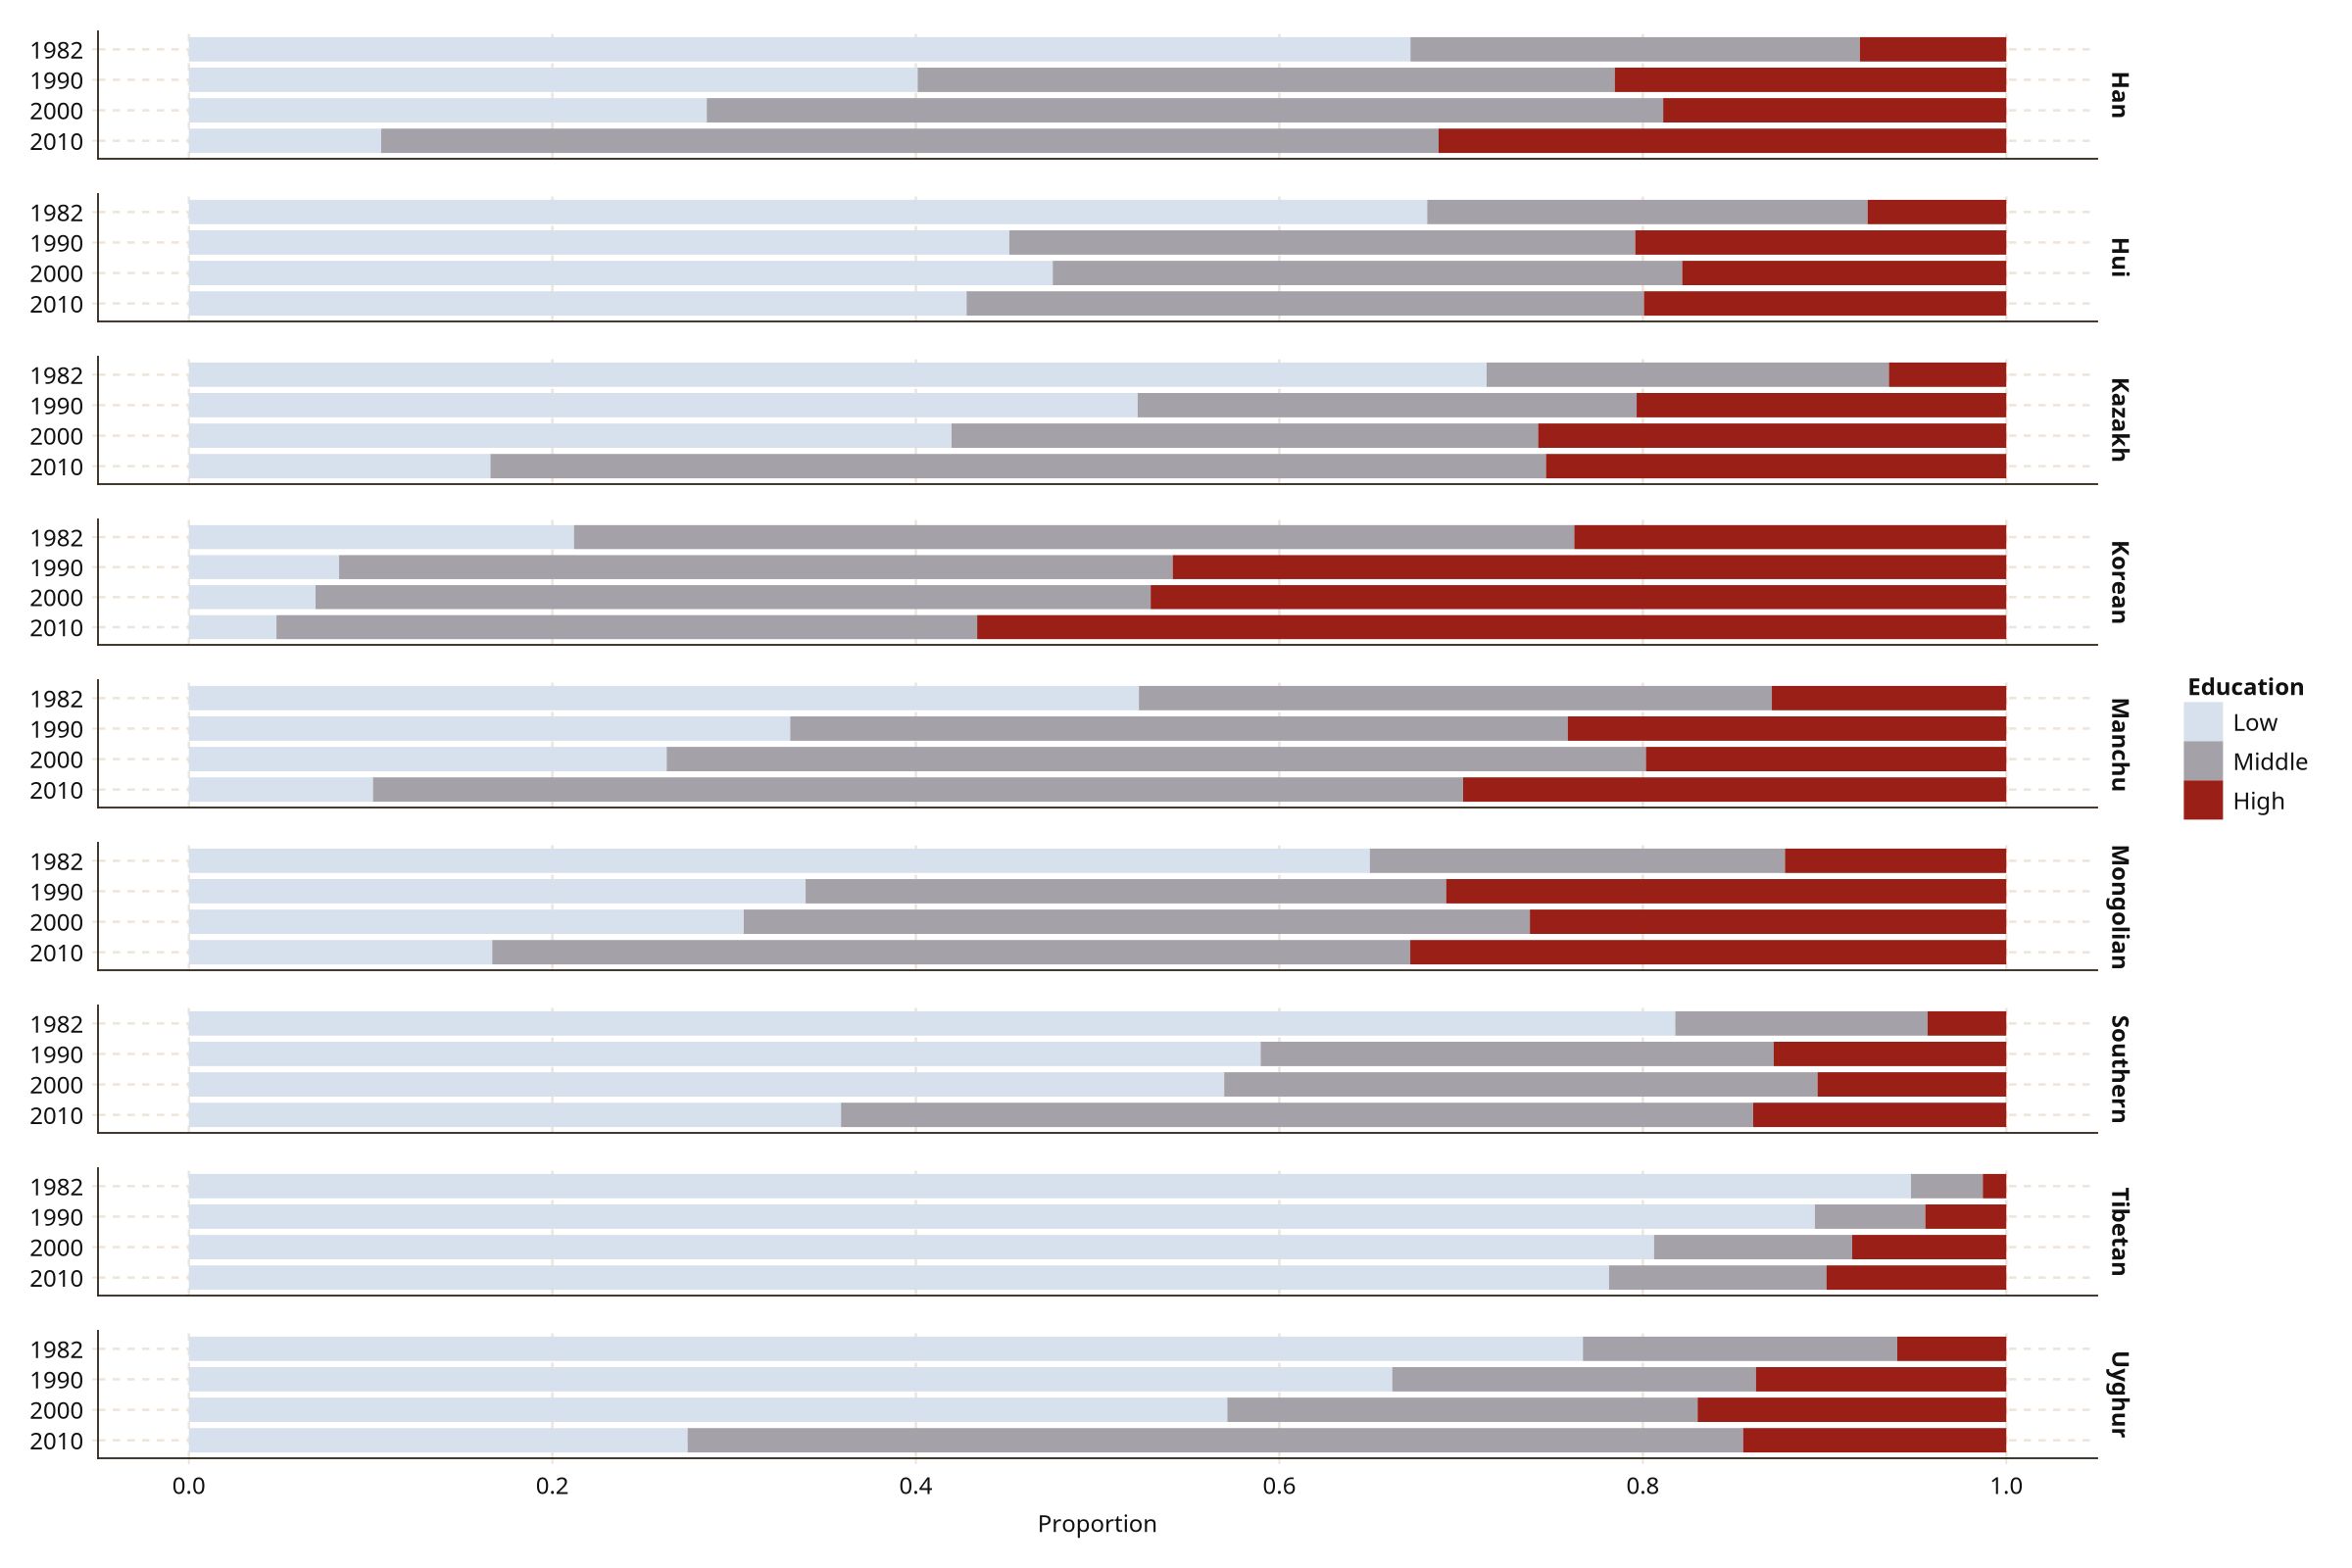
\includegraphics[width=0.7\textwidth]{../graphs/edu_comp.png}
    \caption{Educational composition across ethnic groups, 1982-2010}
    \label{fig:edu_comp}
\end{figure}

When searching for a partner, achieved status (e.g., education) is often considered alongside ascribed status (e.g., ethnicity)
and has gained greater importance during modernization.
We examine how educational compositions have changed across ethnic groups and whether educational advancement facilitates interethnic marriage.

Figure~\ref{fig:edu_comp} illustrates persistent educational disparities across ethnic groups from 1982 to 2010.
Throughout this period, Koreans remained the most educated group,
with 56.63\% of their married population having completed high school in 2010--nearly double the national average of 29.91\%.
The Manchu, Mongolian, and Han populations followed, each with approximately 30\% of their members holding a high school diploma or higher.

At the lower end of the educational spectrum were the Tibetan, Uyghur, and Southern minorities,
with Tibetans experiencing the greatest disadvantage.
Educational expansion had notably less impact on these groups.
For instance, while the national proportion of individuals with primary education or less dropped to 12.85\% by 2010,
among Tibetans this figure remained at 78.14\%, down from 94.75\% in 1982.
Thus, despite overall educational progress, ethnic disparities in educational attainment widened over time

\begin{figure}[htbp]
    \centering
    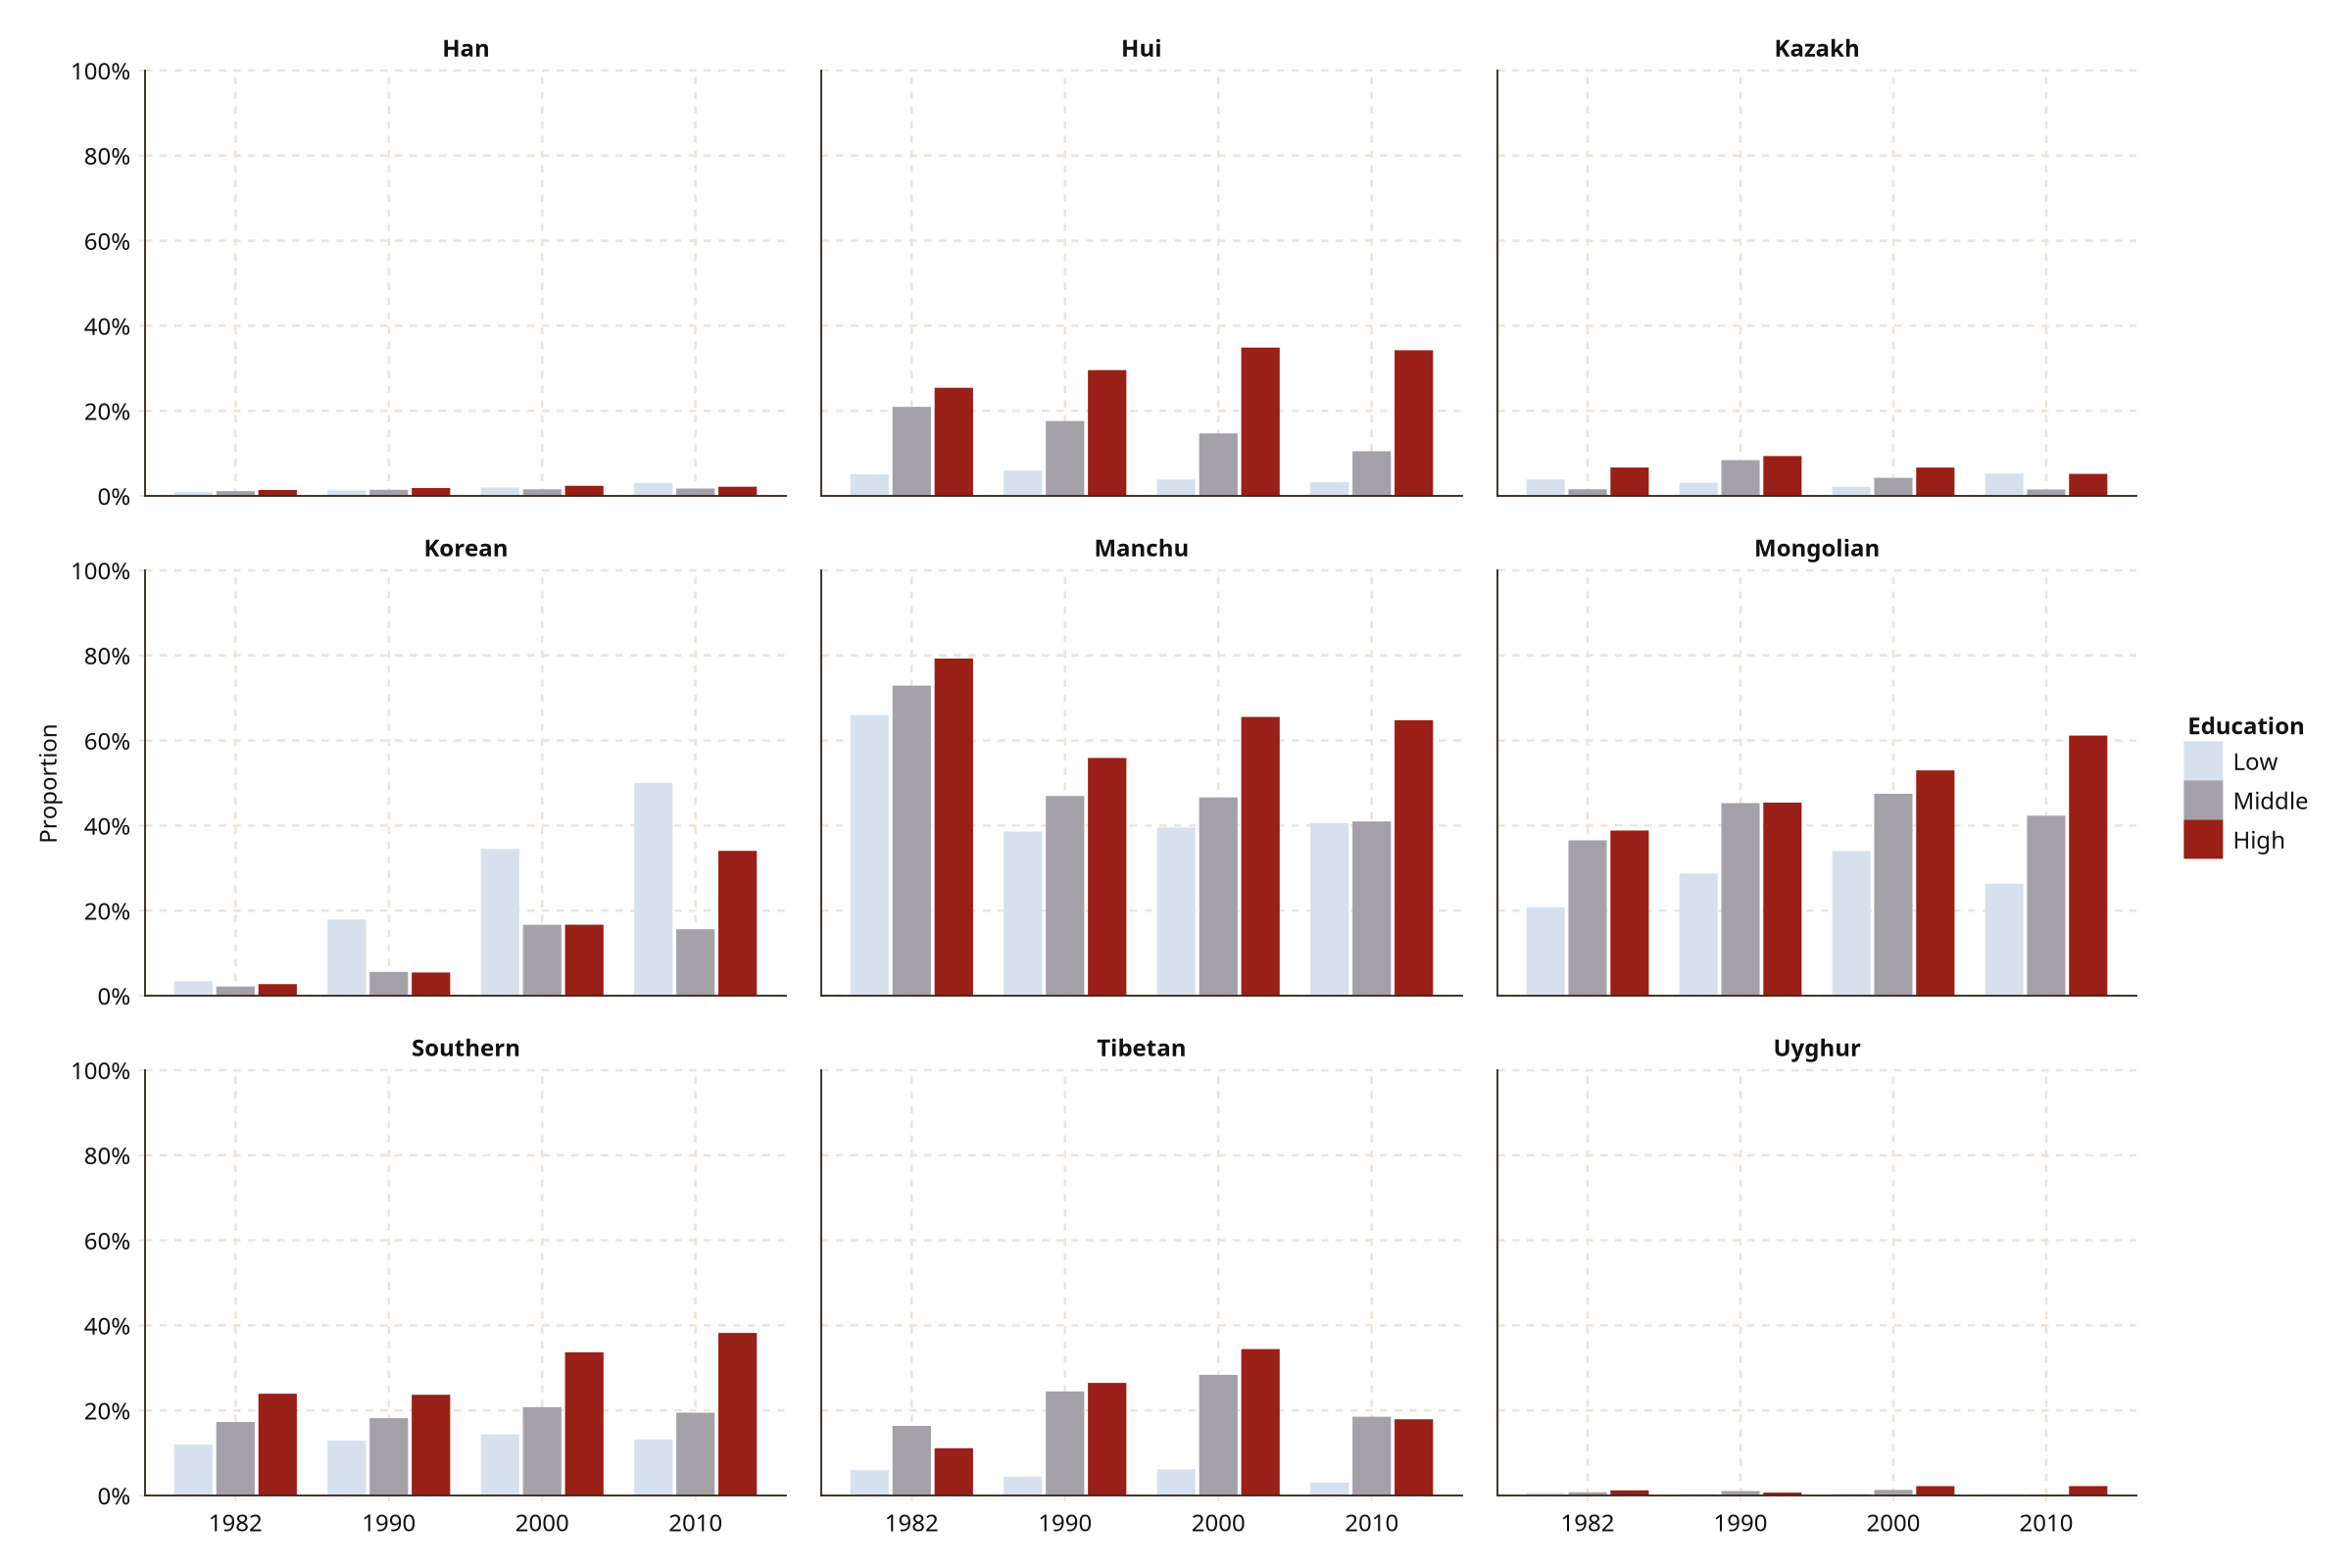
\includegraphics[width=0.7\textwidth]{../graphs/inter_by_edu.png}
    \caption{Proportion of interethnic marriage by educationa and ethnic group, 1982-2010}
    \label{fig:inter_by_edu}
\end{figure}

Figure~\ref{fig:inter_by_edu} illustrates the variation in interethnic marriage rates across educational levels from 1982 to 2010 for each ethnic group.
As shown, there were positive and widening educational gradients in intermarriage rates for the Hui, Manchu, Mongolian, and Southern minorities.
Among the Hui, for example, intermarriage rates in 1982 were 5.11\%, 20.93\%, and 25.42\% for low, middle, and high educational levels, respectively.
By 2010, these rates had shifted to 3.23\%, 10.49\%, and 34.23\%, showing a marked increase in intermarriage among the highly educated.
Similar patterns emerged among the Manchu, Mongolian, and Southern minorities,
where the largest increases--or relatively smaller declines--in intermarriage occurred among those with high school or higher degrees.
The Tibetan population showed less clear educational gradients,
though by 2010, those with middle (18.52\%) or high (17.91\%) school education far exceeded the intermarriage rate of those with low education (3.02\%).

In contrast, the Han majority and Korean populations showed different patterns.
Korean intermarriage rates rose most dramatically among the less educated, from 3.34\% in 1982 to 50\% in 2010,
exceeding the rates for middle (15.63\%) and high (34.04\%) education levels.
Similarly, the Han majority showed higher intermarriage rates
among those with low education (3.04\%) compared to middle (1.73\%) and high (2.15\%) education in 2010.

The Kazakh and Uyghur populations maintained consistently low intermarriage rates across all educational levels.
In 2010, Uyghur intermarriage rates were just 0.29\%, 0.14\%, and 2.21\% for low, middle, and high education levels respectively.

These patterns reveal distinct ethnic differences in how education relates to intermarriage.
While higher education generally corresponds to higher intermarriage rates among the Hui, Manchu, Tibetan, and Southern minorities,
the opposite holds true for Koreans and the Han majority.
The Kazakh and Uyghur populations show minimal intermarriage regardless of education level,
suggesting that ethnic boundaries for these groups remained rigid and largely uninfluenced by instrumental considerations.

